\bookchapter{Errors, Iterators, Modules and Tests}\label{ch:rust5}

\section*{Explanation}
Four tools turn small Rust programs into real software: a way to handle things that can go wrong (errors), a way to process sequences concisely (iterators and closures), a way to organise code in files (modules and crates), and a way to check that it works (tests). All four are different from Python in a way that you will like once you have seen it.

\section*{Errors without exceptions}
Python raises an \emph{exception} that flies up the call stack until somebody catches it, or the program ends. A function does not say in its signature that it may fail. Rust has no exceptions. A function that can fail returns a \textbf{\texttt{Result}}, an enum like \verb!Option!:
\begin{center}
\verb!enum Result<T, E> { Ok(T), Err(E) }!
\end{center}
\verb!Ok(value)! is the success, \verb!Err(error)! the failure, and the type of the function tells every reader that it can fail.
%rs:result
\begin{verbatim}
use std::num::ParseFloatError;

fn parse_voltage(s: &str) -> Result<f64, ParseFloatError> {
    let v: f64 = s.trim().parse()?;       // ? : return the error if any
    Ok(v)
}

fn main() {
    println!("{:?}", parse_voltage(" 24.8 "));
    println!("{:?}", parse_voltage("abc"));
    match parse_voltage("12,5") {
        Ok(v) => println!("ok {v}"),
        Err(e) => println!("error: {e}"),
    }
}
\end{verbatim}
prints
\begin{verbatim}
Ok(24.8)
Err(ParseFloatError { kind: Invalid })
error: invalid float literal
\end{verbatim}
The operator \textbf{\texttt{?}} is the workhorse: if the result is \verb!Ok(v)! it gives you \verb!v!; if it is \verb!Err(e)! the function returns this error immediately to its caller. It replaces the \verb!try/except! pyramids of Python by one character, and the error is always visible in the type. The compiler warns when you ignore a \verb!Result!.

Other ways to treat a result: \verb!.unwrap()! (panic on error, fine in examples and tests), \verb!.expect("message")! (panic with your message), \verb!.unwrap_or(default)!, \verb!.ok()! (convert to \verb!Option!), and \verb!match!/\verb!if let! for full control. \textbf{Panic} is for bugs (``this cannot happen''): it stops the thread and prints a message. \textbf{Result} is for things that can happen in a correct program: a missing file, a packet that does not parse, a sensor that does not answer. On the robot, the network is full of the second kind, so your packet decoder must \emph{never} panic on bad input.

\subsection*{Your own error type}
A program with several sources of errors needs one error type that can hold them all. The simplest version is an enum:
%rs:myerror
\begin{verbatim}
use std::fmt;

#[derive(Debug)]
enum ConfigError {
    Missing(String),
    BadNumber(String, std::num::ParseIntError),
}

impl fmt::Display for ConfigError {
    fn fmt(&self, f: &mut fmt::Formatter) -> fmt::Result {
        match self {
            ConfigError::Missing(k) => write!(f, "key '{k}' is missing"),
            ConfigError::BadNumber(k, e) => write!(f, "key '{k}': {e}"),
        }
    }
}

impl std::error::Error for ConfigError {}

fn get_port(pairs: &[(&str, &str)]) -> Result<u16, ConfigError> {
    let (_, v) = pairs.iter().find(|(k, _)| *k == "port")
        .ok_or(ConfigError::Missing("port".to_string()))?;
    let n: u16 = v.parse()
        .map_err(|e| ConfigError::BadNumber("port".into(), e))?;
    Ok(n)
}

fn main() -> Result<(), Box<dyn std::error::Error>> {
    println!("{:?}", get_port(&[("port", "9000")]));
    if let Err(e) = get_port(&[("host", "robot")]) { println!("{e}"); }
    if let Err(e) = get_port(&[("port", "99999")]) { println!("{e}"); }
    let p = get_port(&[("port", "x")])?;     // main returns the error
    println!("unreachable {p}");
    Ok(())
}
\end{verbatim}
prints \verb!Ok(9000)!, \verb!key 'port' is missing! and \verb!key 'port': number too large to fit in target type!. The last call returns the error from \verb!main!, so the program ends with exit code $1$ and the message \verb!Error: BadNumber("port", ParseIntError { kind: InvalidDigit })! on standard error. \verb!Box<dyn Error>! is a convenient return type for \verb!main! and for small tools: any error type can be converted into it with \verb!?!. For big programs, the crates \verb!thiserror! (library errors) and \verb!anyhow! (application errors) remove the boilerplate of the \verb!impl! blocks; they are used in most Rust projects.

\section*{Closures and iterators}
A \textbf{closure} is a small anonymous function, written \verb!|x| x * 2! (Python: \verb!lambda x: x * 2!), which may use variables of its surroundings. An \textbf{iterator} produces a sequence of values one at a time. Iterators can be chained with methods like \verb!map!, \verb!filter!, \verb!sum!, \verb!zip!, \verb!enumerate!, \verb!rev!, \verb!take!, \verb!collect!, as comprehensions in Python, but in a pipeline. The pipeline is \emph{lazy}: nothing happens until a final step (\verb!sum!, \verb!collect!, a \verb!for! loop) asks for the values.
%rs:iter
\begin{verbatim}
fn main() {
    let d = vec![0.8, 2.5, 1.1, 3.9, 0.3];
    let near: Vec<f64> = d.iter().copied().filter(|&x| x < 1.5).collect();
    let total: f64 = d.iter().sum();
    let doubled: Vec<f64> = d.iter().map(|x| x * 2.0).collect();
    let mx = d.iter().cloned().fold(f64::MIN, f64::max);
    let idx = d.iter().position(|&x| x == mx);
    let pairs: Vec<(f64, f64)> =
        d.iter().copied().zip(d.iter().skip(1).copied()).collect();
    let diffs: Vec<f64> = d.windows(2).map(|w| w[1] - w[0]).collect();
    println!("{near:?} {total:.1}");
    println!("{doubled:?}");
    println!("{mx} {idx:?} {}", pairs.len());
    println!("{diffs:.1?}");
    let any_close = d.iter().any(|&x| x < 0.5);
    let all_pos = d.iter().all(|&x| x > 0.0);
    println!("{any_close} {all_pos}");
}
\end{verbatim}
prints
\begin{verbatim}
[0.8, 1.1, 0.3] 8.6
[1.6, 5.0, 2.2, 7.8, 0.6]
3.9 Some(3) 4
[1.7, -1.4, 2.8, -3.6]
true true
\end{verbatim}
In Python the same lines are list comprehensions or \verb!sum(...)!; the Rust versions are as short, and because they are compiled with the whole pipeline in view they are normally \emph{as fast as a hand-written loop} (``zero-cost abstraction''; in a debug build they are much slower, Chapter~\ref{ch:rust1}). \verb!iter()! borrows the elements, \verb!iter_mut()! lets you change them, \verb!into_iter()! consumes the vector (Chapter~\ref{ch:rust3}). You can also write your own iterator by implementing the trait \verb!Iterator! with one method, \verb!next!.

\section*{Maps and sets}
\verb!HashMap<K, V>! is the \verb!dict!, \verb!HashSet<T>! the \verb!set!. Looking up gives an \verb!Option!, because the key may be missing.
%rs:map
\begin{verbatim}
use std::collections::HashMap;

fn main() {
    let mut battery: HashMap<String, f64> = HashMap::new();
    battery.insert("robot1".to_string(), 24.1);
    battery.insert("robot2".to_string(), 21.7);
    *battery.entry("robot2".to_string()).or_insert(0.0) -= 0.5;
    println!("{:?}", battery.get("robot2"));
    println!("{:?}", battery.get("robot9"));
    let mut names: Vec<_> = battery.keys().cloned().collect();
    names.sort();
    println!("{names:?}");
}
\end{verbatim}
prints \verb!Some(21.2)!, \verb!None! and \verb!["robot1", "robot2"]!. The order of a \verb!HashMap! is not defined (different from the \verb!dict! of Python, which keeps the order of insertion); use a \verb!BTreeMap! for sorted order. The \verb!entry! method means ``find it or insert it'' in one step.

\section*{Modules, crates and the file layout}
Every file can be a \textbf{module}. In \verb!src/main.rs!:
\begin{verbatim}
mod protocol;            // the code is in src/protocol.rs
mod sensors { pub fn read() -> f64 { 0.0 } }   // or inline

use protocol::Message;   // short name instead of protocol::Message

fn main() {
    let m = Message::new();
    println!("{}", sensors::read());
}
\end{verbatim}
Everything is \textbf{private} by default; \verb!pub! makes an item visible outside its module. A larger project grows like this:
\begin{center}
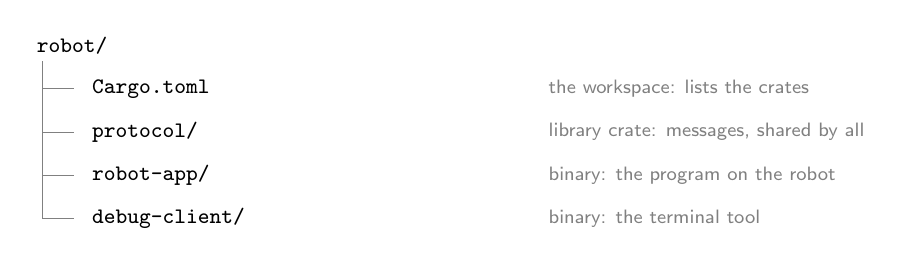
\begin{tikzpicture}[font=\ttfamily\footnotesize]
 \node[anchor=west] at (0,0) {robot/};
 \node[anchor=west] at (0.7,-0.55) {Cargo.toml};  \node[anchor=west,font=\sffamily\scriptsize,gray] at (6.5,-0.55) {the workspace: lists the crates};
 \node[anchor=west] at (0.7,-1.1) {protocol/};   \node[anchor=west,font=\sffamily\scriptsize,gray] at (6.5,-1.1) {library crate: messages, shared by all};
 \node[anchor=west] at (0.7,-1.65) {robot-app/};  \node[anchor=west,font=\sffamily\scriptsize,gray] at (6.5,-1.65) {binary: the program on the robot};
 \node[anchor=west] at (0.7,-2.2) {debug-client/}; \node[anchor=west,font=\sffamily\scriptsize,gray] at (6.5,-2.2) {binary: the terminal tool};
 \draw[gray] (0.2,-0.2)--(0.2,-2.2) (0.2,-0.55)--(0.6,-0.55) (0.2,-1.1)--(0.6,-1.1) (0.2,-1.65)--(0.6,-1.65) (0.2,-2.2)--(0.6,-2.2);
\end{tikzpicture}
\captionof{figure}{A \emph{workspace} with a shared library crate and two programs. The robot and the client use exactly the same message definitions, so they cannot disagree.}
\end{center}
A workspace has a top-level \verb!Cargo.toml!:
\begin{verbatim}
[workspace]
members = ["protocol", "robot-app", "debug-client"]
resolver = "3"
\end{verbatim}
and each member lists what it needs, e.g.\ \verb!protocol = { path = "../protocol" }! under \verb![dependencies]!. External crates come from \verb!crates.io!: \verb!cargo add serde! (or an entry such as \verb!rand = "0.9"!). Cargo downloads the crate and everything it depends on and records the exact versions in \verb!Cargo.lock!. Commit \verb!Cargo.lock! for programs, so every build uses the same versions. Libraries on \verb!crates.io! are documented on \verb!docs.rs!; \verb!cargo doc --open! builds the documentation of your own project. Comments that start with \verb!///! become documentation.

\section*{Tests}
Tests live next to the code and are run with \verb!cargo test!. No framework to install and nothing to import, as in Chapter~\ref{ch:py11}.
%rslib:tests
\begin{verbatim}
pub fn wrap_angle(deg: f64) -> f64 {
    (deg + 180.0).rem_euclid(360.0) - 180.0
}

#[cfg(test)]
mod tests {
    use super::*;

    #[test]
    fn inside_range_is_unchanged() {
        assert_eq!(wrap_angle(45.0), 45.0);
    }

    #[test]
    fn wraps_both_directions() {
        assert!((wrap_angle(190.0) - (-170.0)).abs() < 1e-9);
        assert!((wrap_angle(-190.0) - 170.0).abs() < 1e-9);
    }

    #[test]
    #[should_panic]
    fn unwrap_none_panics() {
        let v: Option<f64> = None;
        v.unwrap();
    }
}
\end{verbatim}
\verb!cargo test! prints
\begin{verbatim}
running 3 tests
test tests::inside_range_is_unchanged ... ok
test tests::wraps_both_directions ... ok
test tests::unwrap_none_panics - should panic ... ok

test result: ok. 3 passed; 0 failed; 0 ignored
\end{verbatim}
\verb|assert!(condition)| and \verb|assert_eq!(a, b)| stop the test with a message if they are false; for floating-point numbers compare with a tolerance (Chapter~\ref{ch:py2}), never with \verb!==!. The block \verb!#[cfg(test)]! is only compiled for tests. Larger test programs go to a folder \verb!tests/! next to \verb!src/!. Code examples in the documentation comments are also run as tests (\emph{doctests}).

\section*{Formatting, linting, and what to run before a commit}
\begin{center}
\renewcommand{\arraystretch}{1.2}
\begin{tabular}{lp{8.6cm}}
\verb!cargo fmt! & one standard formatting; no more arguments about style\\
\verb!cargo clippy! & hundreds of suggestions: ``use \verb!.is_empty()!'', ``this clone is not needed''\\
\verb!cargo test! & all tests\\
\verb!cargo build --release! & the build that goes to the robot\\
\end{tabular}
\end{center}
Make these the first four steps of the continuous integration (CI) of your repository (Chapter~\ref{ch:git3} for the tools); a pull request is only merged when all four pass.

\begin{aibox}[The robot never panics]
For the program on the robot, decide the policy: a panic on the control thread stops the robot, so the production code treats everything that comes from outside (network packets, files, sensor values) as untrusted and returns \verb!Result! or \verb!Option!. \verb!unwrap()! and array indexing with an unchecked index are fine in tests and for conditions that you have just checked, but each one in the main loop is a possible crash in the middle of a match. Search your code for \verb!unwrap! before the competition.
\end{aibox}

\section*{Practice problems}
\begin{enumerate}[label=\textbf{\thechapter.\arabic*}]
  \item What is the difference between a function that returns \verb!Option<T>! and one that returns \verb!Result<T, E>!? Give one example for each from the robot.
  \item Write \verb!fn parse_pair(s: &str) -> Result<(f64, f64), std::num::ParseFloatError>! that parses \verb!"1.5,-2"! into the pair $(1.5,-2.0)$ using \verb!?!. What happens with \verb!"1.5"!? (Think: which iterator method gives a missing second part, and what do you do with it?)
  \item Use iterators to compute from a \verb!Vec<f64>! of distances: (a) the number of values in $[0.5,2.0]$, (b) the mean of the values above $1$, (c) the vector of squares.
  \item Given $xs$ and $ys$ as two vectors of equal length, compute the dot product $\sum x_iy_i$ with \verb!zip!. Compare the result for $(1,2,3)\cdot(4,5,6)$ with Chapter~\ref{ch:dotproduct}.
  \item Write a function \verb!moving_average(xs: &[f64], n: usize) -> Vec<f64>! using \verb!windows!. Test with $[1,2,3,4,5]$ and $n=3$.
  \item Count how often each word appears in a text with a \verb!HashMap!. Print the words sorted by count (highest first), ties alphabetically.
  \item Which of these is a bug that should be a \verb!panic!, and which an error that should be a \verb!Result!? (a) a packet from the network with a wrong checksum, (b) an array index that must be below $22$ by construction of the program, (c) the file \verb!config.toml! does not exist, (d) \verb!divide(a, b)! with $b=0$ in a function whose documentation says $b\neq0$, (e) the camera does not deliver a frame.
  \item Write tests for a function \verb!fn clamp(x: f64, lo: f64, hi: f64) -> f64! with three cases (inside, below, above) and one test that checks the case $lo>hi$ (decide what the right behaviour is and write it into the documentation comment).
  \item Create a workspace with a library crate \verb!geometry! (with a function \verb!distance!) and a binary crate \verb!app! that uses it. Which lines do you need in the two \verb!Cargo.toml! files?
  \item[\textbf{\thechapter.10}$\star$] Write a function that reads a CSV text with the lines \verb!time,x! (header first) into a \verb!Vec<(f64, f64)>!, returns an error with the line number for a line that does not have two numbers, and skips empty lines. Write tests for a good file, for a line with a text instead of a number, and for an empty file. Use your own error enum with \verb!Display!.
\end{enumerate}
